% Files using this must be two subfolders
% deep. Adjust the number of ../ for the
% depth of the file.
% Imports
\usepackage{fancyhdr}
\usepackage{geometry}
\usepackage{icomma}
\usepackage{amsmath}
\usepackage{multicol}
\usepackage{mathptmx}
\usepackage{anyfontsize}
\usepackage{t1enc}
\usepackage{tabto}
\usepackage{listings}
\usepackage{filecontents}
\usepackage{subcaption}
\usepackage{tikz}
\usepackage[parfill]{parskip}
\usepackage{graphicx}
\usepackage[]{mdframed}
\usepackage{amsmath}
\usepackage[makeroom]{cancel}
\usepackage{pgfplots}
\usepackage{pgfplotstable}
\usepackage{xfrac}
\usepackage{amssymb}
\usepackage{mathtools}
\pgfplotsset{compat=1.18}
\usetikzlibrary{patterns}
\usepgfplotslibrary{polar}
\usepgfplotslibrary{fillbetween}

\geometry{margin=2.5cm}

\newcommand{\name}{Kaleb Burris}
\newcommand{\classname}{MATH F253, Elizabeth S. Allman, University of Alaska Fairbanks}
\newcommand{\assignment}{FILL IN ASSIGNMENT NAME}

\pagestyle{fancy}

\fancyhead[L]{
    \name 
    \newline
    \classname
    \newline
    \assignment
}

\newcommand{\horizontal}{\noindent\rule{\hsize}{0.4pt}}

\setlength{\headheight}{42pt}
\setlength{\headsep}{0.25in}
\setlength{\columnsep}{0.35cm}
\setlength{\columnseprule}{1pt}

\usepackage[T1]{fontenc}
\usepackage{lmodern}

\usepackage{enumitem}
\usepackage{graphicx}
\graphicspath{ {./lab06images/} }

% Put class number, class name, and professor 
% name.
% Use only in case of emergency, this
% should be covered by the preamble.
% \renewcommand\classname{}

% Put the assignment name with \S if 
% necessary for the section and the question 
% numbers.
\renewcommand\assignment{Lab 6: Momentum, 3/7/2023, Partners: Maite Valentin-Lugo, Seth Waln}

\begin{document}

    % Templates
    \iffalse
    % Use these for equations.
    \begin{equation*}
        \begin{gathered}
            Equations go here.
        \end{gathered}
    \end{equation*}

    % Use this if a line of math is too long.
    \resizebox{\hsize}{!}{$Long equation goes here$}

    % Use these for multiple columns.
    \begin{multicol*}{# of columns}
        % Remove the * if you want the columns to be balanced.
    \end{multicol*}

    % Use this to add a horizontal line.
    \horizontal

    \fi

    % Begin homework here.
    %%%%%%%%%%%%%%%%%%%%%%

    \section*{Part 1}

    \paragraph*{1.}
    \begin{equation}
        \vec{p} = m\vec{v}
    \end{equation}

    Momentum is derived as the mass of an object times its velocity.

    \begin{equation}
        \vec{F_{net}} = \frac{d\vec{p}}{dt}
    \end{equation}

    The net force of a system is the rate of change of the momentum.

    \begin{equation}
        \vec{p_{i}} = m_{1}\vec{v_{1f}} + m_{2}\vec{v_{2f}}
    \end{equation}

    The total momentum of a system where an elastic collision occurs is the sum of the masses times their velocities, both at the beginning and at the end.

    \paragraph*{2.}
    The small glider will move back in the direction it came and the large glider will travel with a smaller magnitude to the right than the mall glider initially had.

    \paragraph*{3.}
    The experiment mimicked what I guessed would happen.

    \paragraph*{4.}\mbox{}

    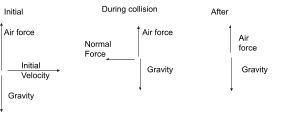
\includegraphics[width=0.8\textwidth]{image5.png}

    \paragraph*{5.}

    The larger glider had a larger velocity after the collision.

    \paragraph*{6.}

    The smaller glider has a much larger velocity after the collision than the larger glider.

    \paragraph*{7.}

    The gliders will stick together and travel at a reduced velocity.

    \paragraph*{8.}

    The results were as predicted, although the nature of the tape caused some strange behavior between the carts on impact.

    \pagebreak

    \paragraph*{9.}\mbox{}

    {\centering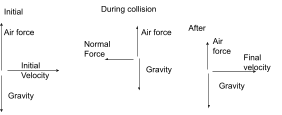
\includegraphics[width=0.8\textwidth]{image12.png}}

    \paragraph*{10.}

    Larger cart: 0.7321 kg

    Smaller cart: 0.5223 kg

    \paragraph*{11.}\mbox{}

    {\centering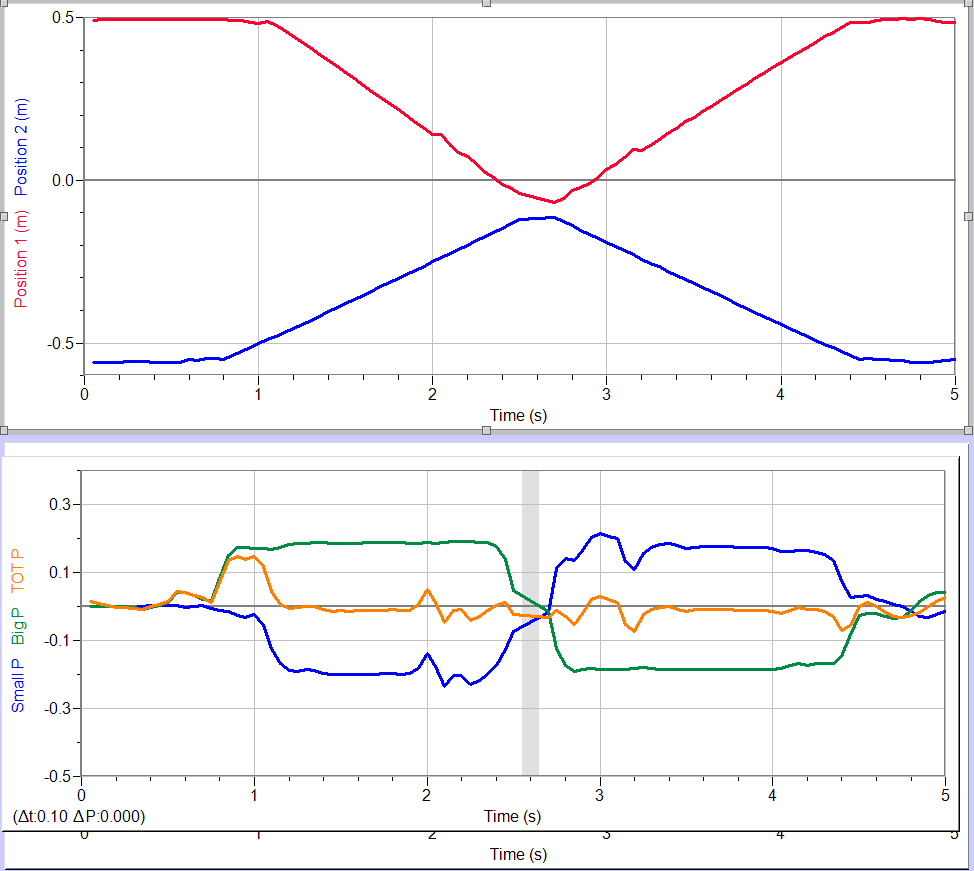
\includegraphics[width=0.8\textwidth]{image4.png}}

    Momentum was conserved as the total P was not noticeably reduced after the collision.

    \paragraph*{12., 13., 14.}

    {\centering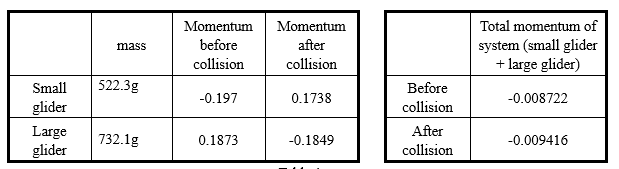
\includegraphics[width=0.8\textwidth]{image13.png}}

    The total P after the collision was the negative of the total initial momentum, with a relatively small margin of error.

    \paragraph*{15.}

    {\centering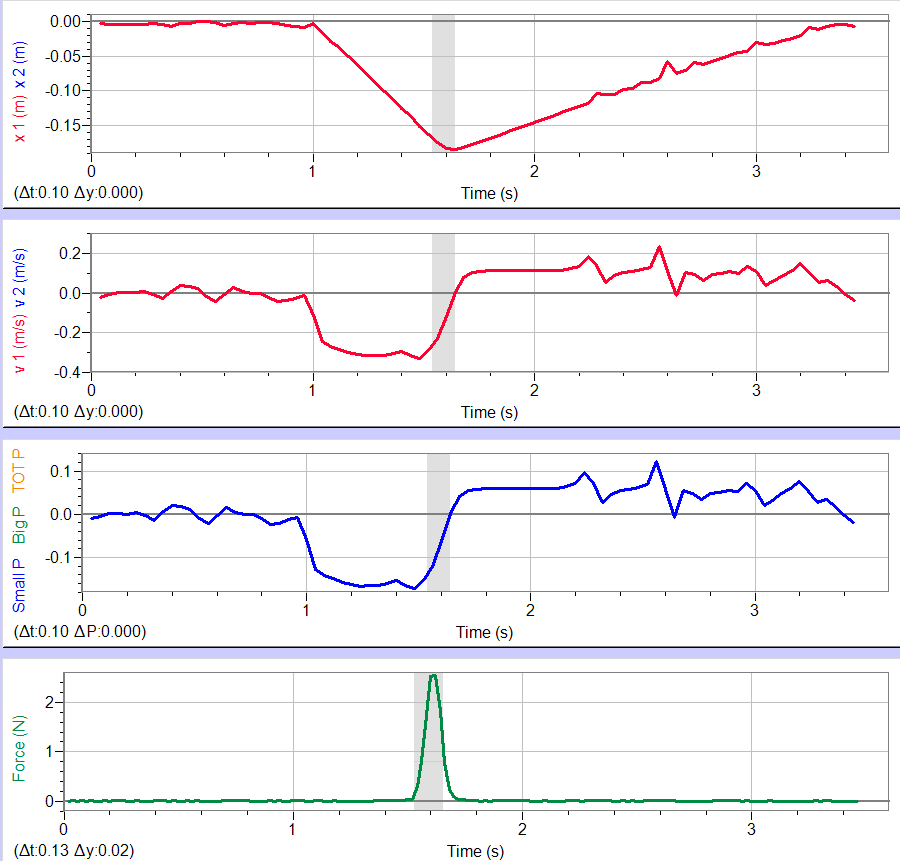
\includegraphics[width=0.8\textwidth]{image11.png}}

    \paragraph*{16.}\mbox{}\\

    Initial: -0.3058m/s * 0.5223kg = -0.1597 (kg*m)/s
    
    Final: 0.113m/s*0.5223kg = 0.0590 (kg*m)/s

    0.0590 - -0.1597 = 0.2187 N*s

    \paragraph*{17.}

    Integral for: Latest | Force
    
    Integral: 0.2213 N*s

    \paragraph*{18.}

    In order for momentum to be conserved, there must be no way the system can leak energy out of itself, such as through air resistance or friction.

    \paragraph*{19.}

    The force itself on the carts was the same, although because of the difference in mass, both carts were left with a final velocity that was different in magnitude from each other.

    \paragraph*{20.}

    No, momentum was not conserved as the magnitude of both momentums after the collision were both lower than the momentum before the collision, thus a leak of energy occurred and the system did not conserve its momentum.

    \paragraph*{21.}

    The mass of the carts, the inaccuracy of the sensor, and the several external forces such as air resistance all act as sources of uncertainty.

    \paragraph*{22.}

    The force between the cart and the force probe was the same.

    \paragraph*{23.}

    The $\Delta p$ was 0.3\%. Because of the stability of the data measurements and sheer volume of data it's working on, the one derived from force.

\end{document}